The first section of this chapter deals with the resources used for the project, while the subsequent ones focuse completely on setting up the CFD software tools and executing the actual simulation. The subchapters are splitted up according to the different parts of software or properties, which they deal with.
\section{Technology used}
CFD is an area with huge demands in terms of resoucres. Therefore industrial CFD calculations belong to the domain of supercomputers or HPCCs (high performance computing clusters). Fortunatelly everything needed for the conduction of this project was provided in the FH Joanneum facility and will be discussed in the following.
\subsection{Hardware}
The department of Aviation at the University of Applied Sciences in Graz is equipped with a HPC (high performance computing) laboratory, compromising sixteen high performance computers, capable of providing the huge amount of CPU power needed for CFD calculations.

For conducting the calculation a cluster of six machines of the model described in table \ref{tab:hardwarespec} were used.
\begin{table}[ht]
\centering
\caption{Specification of computing hardware}
\label{tab:hardwarespec}
\begin{tabular}{ll}
Central Processing Unit (CPU)&Intel\textsuperscript{\textregistered} Xeon(R) CPU X5690\\
Architecture&x86\underline{\space}64\\
Core speed&1596 MHz\\
Cores&12\\
Random Access Memory (RAM)&23.6 GB\\
\end{tabular}
\end{table}

\subsection{Software}
The computers in the HPC laboratory feature the operating system Debian 7.8 (wheezy). Each has the software packages ANSYS ICEM 14.0 and ANSYS CFX 15.0 installed, which were used for performing the simulation. Additionally minor calculation, as well as the analysis and visualisation of the results was done with MATLAB\textsuperscript{\textregistered}.

\emph{ANSYS ICEM CFD 15.0} is an effective software tool for generating, improving and repairing CAD (Computer Aided Design) meshes. Its primary function however is the generation and enhancement of meshes, which are necessary for the flow simulation. Therfore it allows the import from various different CAD softwares and is able to export the mesh for several different CFD solvers such as ANSYS CFX.
	
ANSYS CFX is the software tool used for conducting the simulation. It is a high-performance CFD program for many different fluid flow problems and comes with a highly potent and intuitive GUI. There are three different subprograms for individual simulation tasks. \emph{ANSYS CFX 14.0 Pre} is responsible for setting up initial conditions, solver settings and the like, while \emph{ANSYS CFX-Solver Manager 14.0} deals with the actual solving of the equations for the indiviual meshes and timesteps. The third one, \emph{ANSYS CFX CFD-Post 14.0}, is used for the post-processing and analysis of finished calculations and is capable of 3D visualization of the results, as well as performing various calculations and drawing charts.

The following subchapters are divided according the the software tool, used for this step.
\section{Mesh generation with Ansys ICEM 14.0}
The meshed NACA 0012 airfoil was provided as two-dimensional C-grid mesh by Dr. Wolfgang Hassler as it can be seen in fig. \ref{fig:init_mesh}. It is meshed with hexahedral elements and features a total of 219,000 elements. The domain shows physical meassurements of 7m by 5m by 0.01m and the wing profile inside the domain comes with a chord length of 1m. Due to the nature of the profile with maximum thickness of 12\% the thickness would therefore be 0.12m in total values. On the left side is located the inlet, on the right the outlet and the upper and lower borders are defined as walls, as you can see in figure \ref{fig:init_mesh}. Figure \ref{fig:mesh_closeup} shows the massive grid refinement at the airfoil surface.
\begin{figure}[ht]
\centering
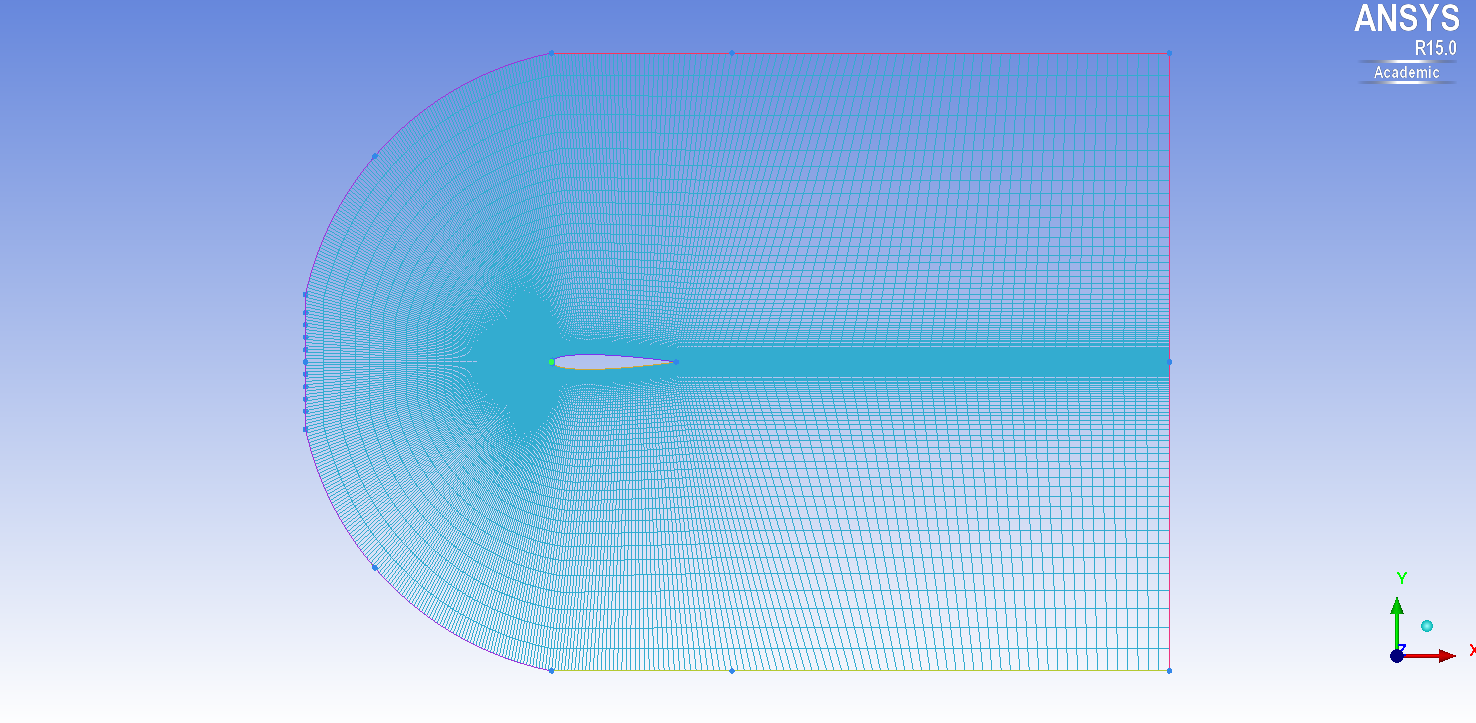
\includegraphics[scale=0.3]{initial_geometry_1.png}
\caption{Provided domain with mesh refinement in viscinity of the wing surface}
\label{fig:init_mesh}
\end{figure}

\begin{figure}[ht]
\centering
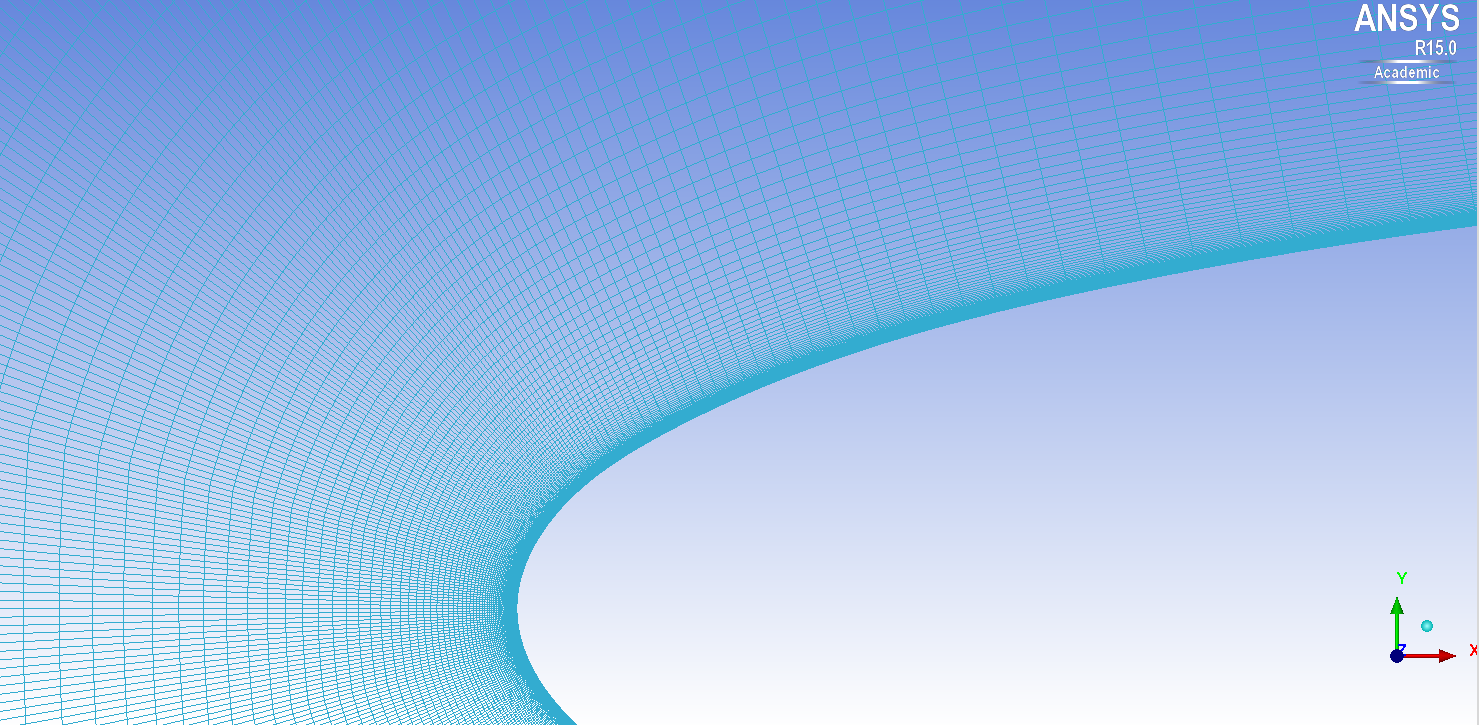
\includegraphics[scale=0.3]{initial_mesh_3.png}
\caption{Closeup to the mesh at the airfoil surface}
\label{fig:mesh_closeup}
\end{figure}

Due to the three-dimensional characteristics of the large eddies this two-dimensional mesh was not sufficient, but had to be extended in the third dimenstion, in order to be capable of providing convincing results. This was achieved by simply extending the given mesh in the third direction by thirty elements, resulting in a physical thickness of 0.30m in z-direction. This leads to a total of 2,263,000 elements and 2,172,810 nodes. In figure \ref{fig:mesh_iso} the final mesh is visible in an isometric view with a closeup of the airfoil.The properties of the final mesh, as it was exported from Ansys ICEM 15.0 are listed in table \ref{tab:mesh_prop}.
\begin{figure}[ht]
\centering
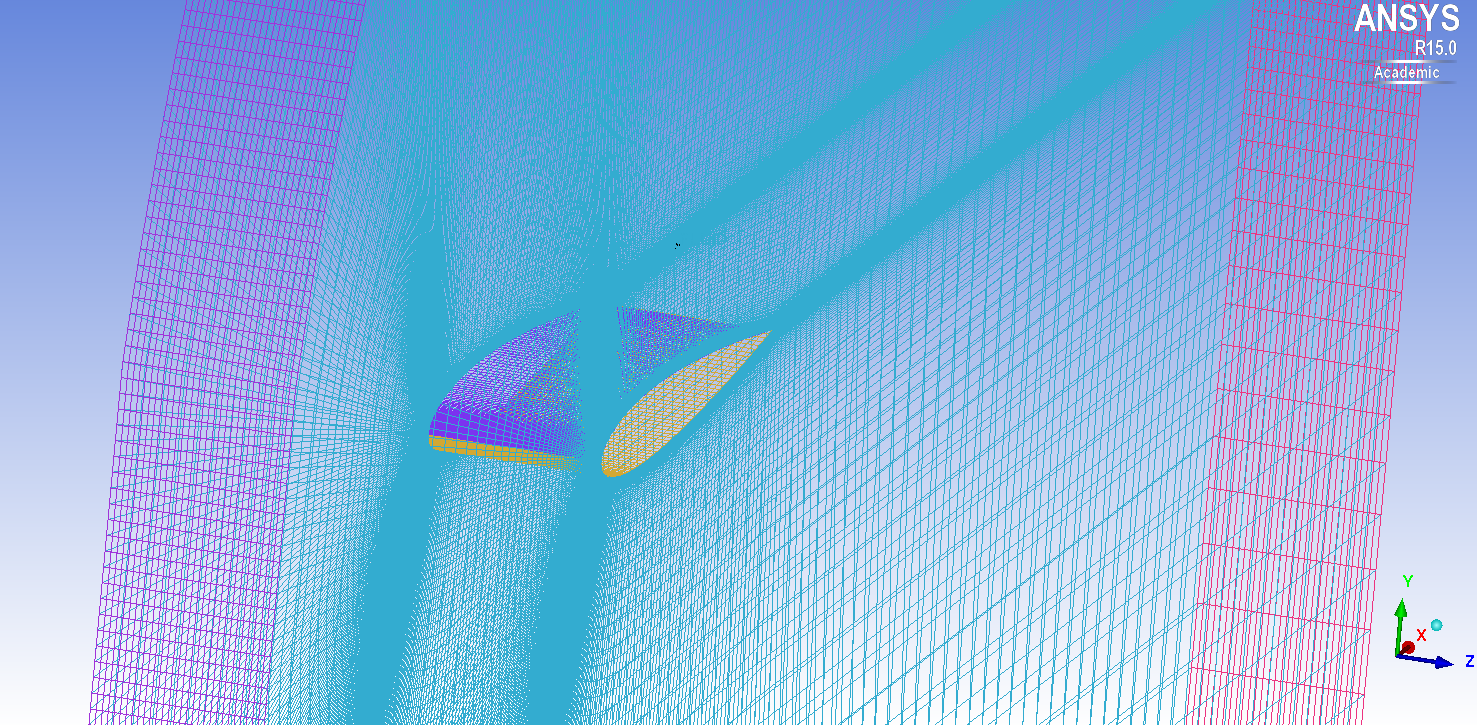
\includegraphics[scale=0.3]{3d_mesh_2.png}
\caption{Closeup of the meshed geometry in isotropic view}
\label{fig:mesh_iso}
\end{figure}
\begin{table}[ht]
\centering
\caption{Properties of the mesh}
\label{tab:mesh_prop}
\begin{tabular}{ll}
Domain length&7m\\
Domain height&5m\\
Domain width&0.3m\\
Profile chord length&1m\\
Maximum profile thickness&0.12m\\
\end{tabular}
\end{table}


\subsection{y\textsuperscript{+} value}
The $y^+$ value is the dimensionless wall distance and an important factor for evaluating the physical accuracy of the flow in viscinity of a wall. It is connected with the frictional velocity $u_{\tau}$ and the kinematic viscosity $\nu$ by
\begin{equation}
\label{eq:yplus}
y^+ = \frac{\rho u_{\tau}y}{\mu}
\end{equation}
with $y$ for the orthogonal offset from the wall. $u_{\tau}$ is then given by
\begin{equation}
u_{\tau} = \sqrt{\frac{\tau_w}{\rho}}
\end{equation}
For the Large Eddy Simulation it is crucial to score a $y^+$ value at around 1.0 or below. In order to evaluate the height of the first cell, necessary to achieve a certain $y^+$ value equation \ref{eq:yplus} can be transformed to
\begin{equation}
\Delta y1 = \frac{y^+ \mu}{\rho u_{\tau}}
\end{equation}  
with the first cell height $\Delta y1$.

The wall shear stress $\tau_w$ can be obtained by the following formula
\begin{equation}
\tau_w = \frac{1}{2} C_f \rho U^2
\end{equation}
with $C_f$ as the skin friction coefficient which must be taken from empirical results. A good estimation for internal flows is $C_f = 0.079 Re^{-0.25}$.

Although the Y+ value is dependend from time and location for simple geometries and flows, such as the one used for this rough estimate, this correlation is highly accurate.

For the calculation of the $\Delta y$ value a short MATLAB\textsuperscript{\textregistered} script has been applied. It yielded a result of 8.02e-6 for the cell in immediate viscinity of the wing surface. An investigation of the given geometry in Ansys ICEM 15.0 (figure \ref{fig:y1_height}) showed that the height of this cell features a cell height of 9.55e-7, which is already beneath the desired value and therefore a refinement of the two-dimensional mesh was not necessary. 
\begin{figure}[ht]
\centering
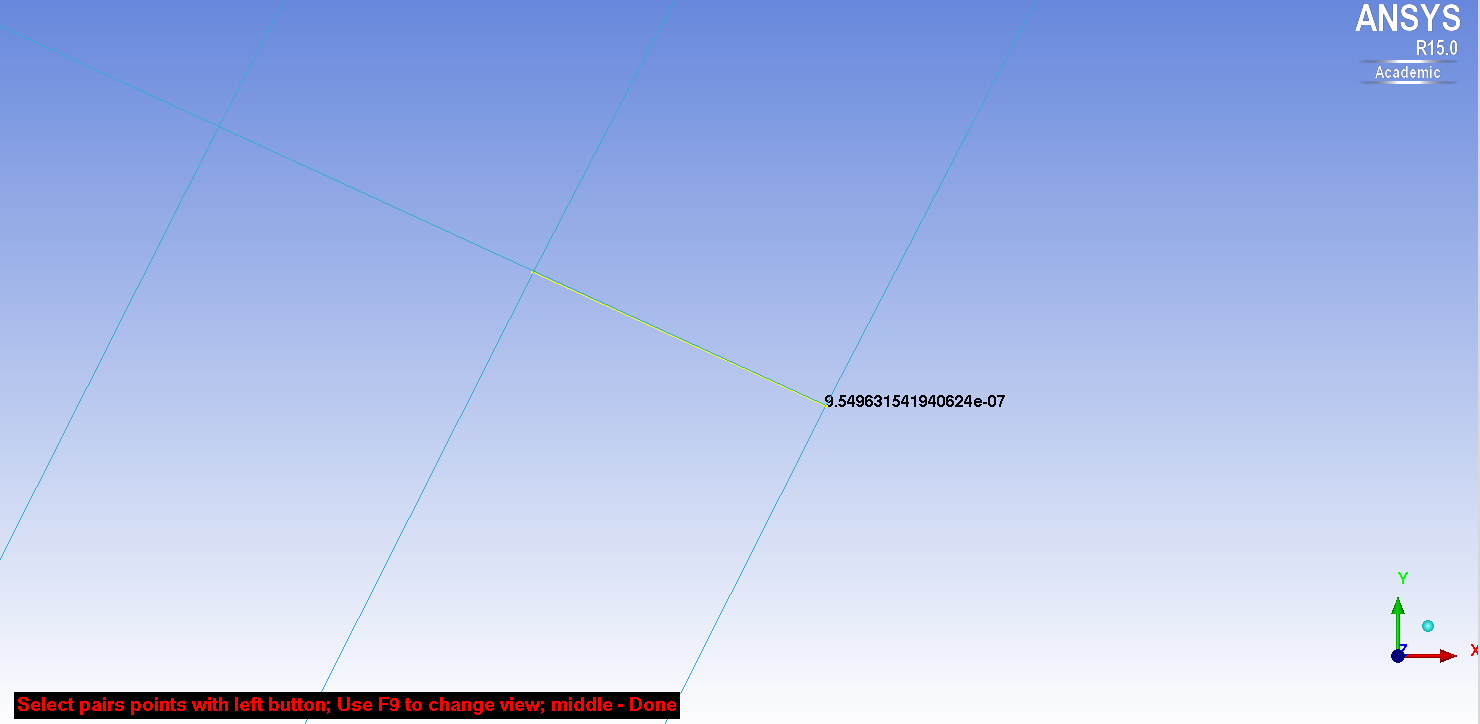
\includegraphics[scale=0.3]{wall_cell.png}
\caption{Meassurement of the height of the cell next to the wing surface}
\label{fig:y1_height}
\end{figure}

\section{Simulation setup in Ansys CFX-Pre 15.0}
There have been two simulations set up in Ansys CFX-Pre, linked together with \emph{Simulation Control}. The first one was a stationary RANS simulation with the task to provide a fully developed flow field as initial condition for the subsequent LES. In Ansys CFX they were entitled according to their simulation type ``Stationary'' and ``Transient''.

Each simulation has the properties described in the the following chapters for themselves. However since they are mostly the same there will be no strict distinction between the two of them, but it will be refered to explicitly, if there have been differences in the adjustment with the different types of simulation.
\subsection{Domain}
The CFD software requires a specific area where the equations for each method can be evaluated. Usually the object of interest is located inside the domain and at the borders of a domain are applied so called boundary conditions, responsible of defining the borders of the area of investigation.
In Ansys CFX one or more fluid models are defined for a domain. These are used to describe and adjust the fluid dominating in this area. For this project only one fluid model was necessary, featuring air at twenty-five degrees.
The turbulence model of the fluid however, was different for stationary- and transient simulation. While the stationary one was based on the $k-\epsilon$ model, the transient applied the LES Smagorinsky model.
\subsection{Analysis type}
For the transient analysis a number of time steps and a value for the time steps themselves had to be considered. For the amount of timesteps an initial amount  of 20,000 was chosen. For adjusting the necessary timestep value the so-called CFL (Courant-Friedrichs-Lewy)number was investigated, which proves to be a good meassurement for accuracy.\\
In order to provide reliable and stable results an average CFL number in the range of 0.5-1.0 is demanded. There are also stable results possible with higher Courant number, but the turbulences may be damped and the result distorted.

After starting the solving with various different timstep values it settled on a value of 1e-5 seconds, which lead to an equivalent Courant number of 0.87.
\subsection{Boundary conditions}
In total there have been seven boundary conditions defined. The first one is for the inlet conditions and provides a constant inlet velocity of 66.8m/s at the western front of the domain. Instead of an outlet, an opening was specified on the eastern border. This is the option of choice for turbulent flows, allowing backflows of the fluid reentering the domain, instead of just leaving. The northern and southern walls were defined as free-slip walls and the wing surface as no-slip wall, leading to a velocity of zero on surface of the wing. Two symmetry conditions at the front- and the backside completed the closure, allowing the domain to stretch out in z-direction hypothetical infinite.
\subsection{Initial conditions}
As inital inlet velocity, 66.8m/s was specified. Furthermore the relative pressure was set to zero, meaning that the initial pressure in the domain equals the pressure prevailing at the outlet.
In Simulation Control it was declared that the LES simulation uses the developed flow field of the preceeding simulation as well.
\subsection{Solver control settings}
For the Advection Scheme for the LES was chosen \emph{Specific Blend Factor}.This scheme allows using a mixture of the High Order Advection Scheme and the CDS (Central Difference Scheme). The relation between these two techniques is controlled via the Blend Factor. For the start a Blend Factor of 0.5 was choosen, meaning that the schemes were used in equal shares. In advance of the solving this factor was altered according to table \ref{tab:blend_factor}, in order to favor more and more the CDS, which would have been the intended choice for the transient simulation. 
Another setting needed for transient simulations is the number of coefficient loops. This is the maximum number of times the equations are iterated for a single timestep.
\begin{quote}
``The implicit coupled solver used in CFX requires the equations to be converged within each timestep to guarantee conservation. The number of coefficient loops required to achieve this is a function of the timestep size. With CFL numbers of order 0.5-1, convergence within each timestep should be achieved quickly. It is advisable to test the sensitivity of the solution to the number of coefficient loops, to avoid using more coefficient loops (and hence longer run times) than necessary.'' – [3]
\end{quote}
As an initial setting the number of maximum coefficient loops has been set to 10. However, if the size of the timestep requires more than tree to five coefficient loops the result can be considered as inaccurate.
As convergence criteria a root mean square of below 1e-6 of the residual target has been demanded. This can be considered as the minimum required accuracy for a LES in order to achieve scientific relevant results.
\begin{table}[ht]
\centering
\caption{Adjustment of the blend factor with respect to the timestep interval}
\label{tab:blend_factor}
\begin{tabular}{ll}
Timestep interval&Blend factor\\
\hline
1 ... 10,000&0.5\\
10,001 ... 15,000&0.3\\
15,001 ... 18,555&0.1\\
\end{tabular}
\end{table}

\subsection{Output control}
Due to numberous timesteps and the resulting large amount of data, only the results of every tenth timestep have been permanently saved to the disk. Furthermore the output of the \emph{Transient Results} have been limited to the properties Pressure, Wall Heat Flux, ?? and the output of the \emph{Transients Stats} to the properties ?? for further decreaseing the necessary storage.
For easy restorage after a shutdown or the like, a full backup has been conducted automatically every hundredth timestep.
\subsection{Simulation control}
The sequence of the simulations and their relationship has been specified by means of the \emph{Simulation Control}. The stationary simulation was executed first with given initial conditions. The transient simulation followed subsequent and was able to benefit from the fully developed flow field of the preceding simulation.
\section{Solving with Ansys CFX-Solver-Manager 15.0}
The solver setup has been specified as full run with double precission checked in order to receive more exact results. The technique of choice was Intel MPI Distributed, which allows the usage of multiple machines on the local network. In total six computers of type described in table \ref{tab:hardwarespec} have been applied for executing the solving.

Due to the provided settings the solver started with the stationary simulation, which finished normally. Thereafter the transient one was conducted. It was aborted after 18,555 timesteps, because a review of the latest results showed that the simulation has already reached a kind of steady state and therefore no more timesteps were needed. In total it took 1.307e6 seconds (15 days, 3 hours, 3 minutes, 58 seconds) to calculate all 18,555 timesteps and writing 1,855 transient result files and 200 backup files.